\section{Motivation}
Hexagonal close-packed (HCP) metals and alloys exhibit a remarkable array of distinct properties, rendering them invaluable across numerous industrial sectors, including nuclear, aerospace, automotive, and bioengineering applications. However, the inherent anisotropic nature arising from their non-symmetric hexagonal crystal lattice significantly influences their deformation behavior, making the fabrication of components from these metals an intricate and costly endeavor. To mitigate manufacturing expenses and to foster more widespread adoption of HCP metals and alloys, developing a comprehensive understanding enabling the accurate modeling of their deformation behavior is imperative.

\vspace{3mm}
Deformation/Mechanical twinning is one of the important contributor in the plastic deformation of HCP metals and alloys. Modeling deformation twinning along with the dislocaton mediated plasticity has been a challenging task. 

\vspace{3mm}
Most models use volume fraction method which is nonphysical \cite{Paduel202111091373}. This approach treats twinning as a diffuse quantity while in reality twinning manifests as a discrete entity. Furthermore, this approach fails to capture the intricate twin morphology within the Representative Volume Element. 

\vspace{3mm}
In the case of deformation kinematics, upon formation, a deformation twin induces a sudden change in shear and it reorients the lattice. Incorporating this sudden transformation needs a distinct approach to handling the kinematics within the constitutive model.

\vspace{3mm}
Many widely used phenomenological models\cite{KALIDINDI1998267} for deformation twinning also omit the stochastic nature of twinning for simplicity. Recent models which use energy based or phase field techniques to model twinning are computationally expensive.

\section{Research Objectives}
The primary objectives of the proposed ``discrete twinning model" are as follows:
\begin{enumerate}
    \item To be computationally efficient yet accurately predict the twin formation.
    \item To model the stochastic nature of twinning.
    \item To capture the physically accurate spatial resolution of a twin which is a discrete entity. 
    \item To capture the morphology of twin nucleation and growth.
    \item To apply the ``sudden" reorientation and shear caused by the twinning at a appropriate timescale in the kinematics of the constitutive law. 
\end{enumerate}

\section{Outline of the thesis}
\begin{itemize}
    \item This chapter contains details about thesis organization and brief introduction to the topic.
    \item Second chapter contains literature review.
    \item Third chapter contains development of new constitutive model for deformation twinning.
    \item Fourth chapter contains model testing.
    \item Fifth chapter contains conclusions and future scope.
\end{itemize}

\section{Brief introduction to the topics}

\subsection{HCP Metals}
The Hexagonal Close Packed (HCP) structure is a densely packed arrangement of equal spheres in a regular, infinite lattice. The HCP unit cell can be envisaged as a hexagonal prism, with an atom at each vertex and three additional atoms at the centre. Alternatively, it can be conceptualised as a stack of three closely packed hexagonal layers(ABA), where the top and bottom layers align.
\begin{figure}[H]
  \centering
  \includesvg[width=3cm]{images/Hexagonal_close_packed.svg}
  \caption{Unit cell structure of HCP [Wikipedia image]}
\end{figure}

Magnesium, Titanium, Zirconium and Beryllium are the most commonly used HCP metals in structural applications, with Hexagonal Close Packed lattice.

\vspace{3mm}
Magnesium and Titanium are known for their excellent \textbf{strength-to-weight ratio} and fatigue resistance, making them ideal for use in various sectors such as automotive, aviation, defence, and spacecraft applications\cite{app11156861}. 

\vspace{3mm}
Titanium and Zirconium, due to their good \textbf{corrosion resistance}, find applications in high-temperature environments like gas turbines and nuclear reactors.

\vspace{3mm}
Beryllium, characterised by its \textbf{low thermal expansion coefficient}, high stiffness, and high strength-to-weight ratio, is used in spacecraft components \cite{Feinberg10.1117/12.924271}. Beryllium is also used as x-ray tubes and lenses, because it is transparent to x-rays and strong enough to hold vacuum \cite{rogers1947high}.

\vspace{3mm}
Titanium and Magnesium, due to their \textbf{compatibility with biological tissues}, are utilised in biomedical applications.

\vspace{3mm}
Beryllium and Zirconium, owing to their very \textbf{low neutron absorption cross-section}, are widely used in the construction of structural components inside a nuclear reactor\cite{Tomberlin_osti_910826}.

\begin{figure}[H]
  \centering
  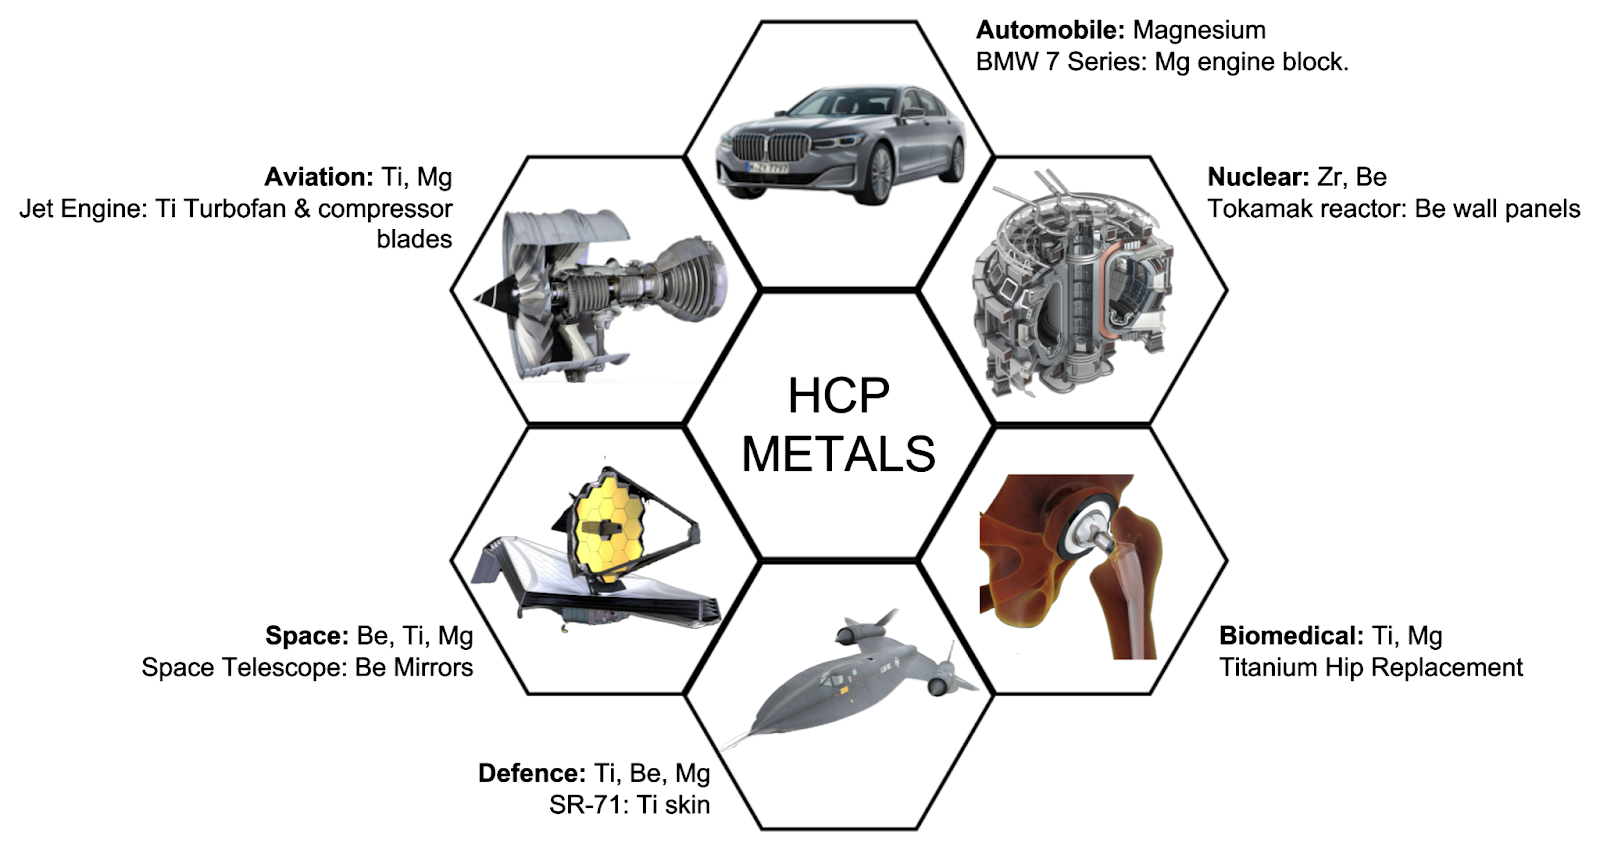
\includegraphics[width=\textwidth]{images/HCP_metals.png}
  \caption{Application of HCP metals in different industrial sectors}
\end{figure}

\vspace{3mm}
However, the widespread use of HCP metals is limited due to the challenges in fabrication, primarily because of their complex deformation behaviour and low ductility. The objective of our study is to gain a deeper understanding of the intricate deformation behaviour of HCP metals, which could potentially enhance manufacturing processes.

\subsection{Twinning}

\begin{figure}[H]
  \centering
  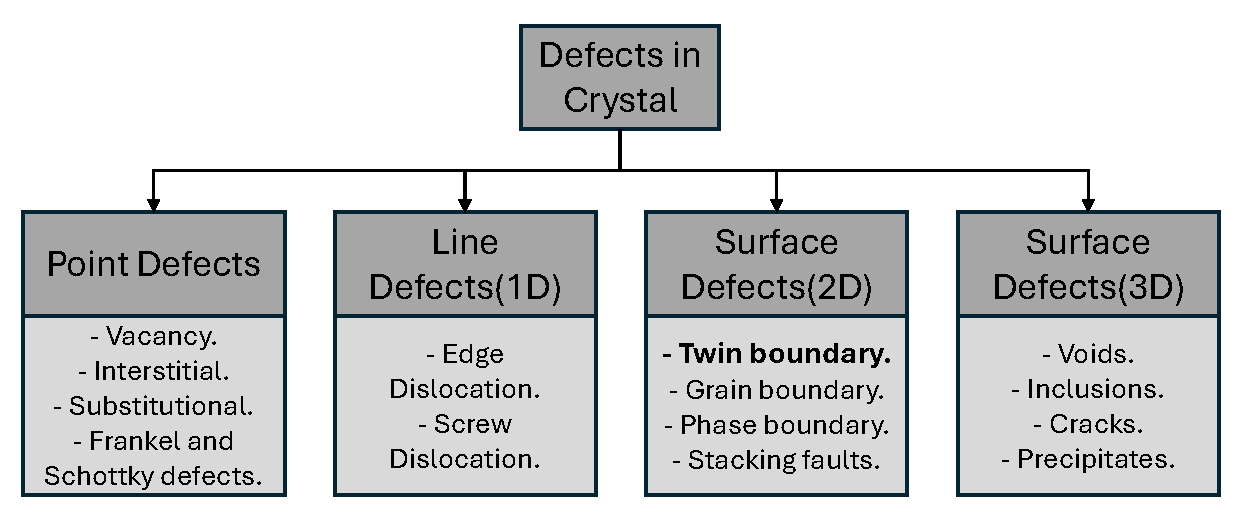
\includegraphics[width=0.8\textwidth]{images/Defects_in_crystals.pdf}
  \caption{Defects in Crystalline Materials.}
  \label{CrystalDefects}
\end{figure}



Twinning is a 2D defect which is characterized by a special form of grain boundary called twin boundary. Twin boundary separates two crystals and at the plane of twin boundary the lattice of two crystals appears to be mirrored as shown in figure \ref{fig:Twinning in 2D}.

\begin{figure}[H]
    \centering
    \resizebox{0.4\textwidth}{!}{
    \begin{circuitikz}
\tikzstyle{every node}=[font=\LARGE]
\draw [short] (11.5,23) -- (2.5,23) ;
\draw [ fill={rgb,255:red,0; green,17; blue,250} ] (2.75,25.25) circle (0.25cm);
\draw [ fill={rgb,255:red,0; green,17; blue,250} ] (5.5,25.25) circle (0.25cm);
\draw [ fill={rgb,255:red,29; green,250; blue,0} ] (4.5,22.25) circle (0.25cm);
\draw [ fill={rgb,255:red,0; green,17; blue,250} ] (3.75,24.5) circle (0.25cm);
\draw [ fill={rgb,255:red,0; green,17; blue,250} ] (5,24.5) circle (0.25cm);
\draw [ fill={rgb,255:red,29; green,250; blue,0} ] (5.25,23) circle (0.25cm);
\draw [ fill={rgb,255:red,0; green,17; blue,250} ] (4.25,25.25) circle (0.25cm);
\draw [ fill={rgb,255:red,0; green,17; blue,250} ] (6.75,25.25) circle (0.25cm);
\draw [ fill={rgb,255:red,0; green,17; blue,250} ] (6.25,24.5) circle (0.25cm);
\draw [ fill={rgb,255:red,0; green,17; blue,250} ] (8,25.25) circle (0.25cm);
\draw [ fill={rgb,255:red,0; green,17; blue,250} ] (4.5,23.75) circle (0.25cm);
\draw [ fill={rgb,255:red,0; green,17; blue,250} ] (10,24.5) circle (0.25cm);
\draw [ fill={rgb,255:red,0; green,17; blue,250} ] (7.5,24.5) circle (0.25cm);
\draw [ fill={rgb,255:red,0; green,17; blue,250} ] (9.25,25.25) circle (0.25cm);
\draw [ fill={rgb,255:red,0; green,17; blue,250} ] (5.75,23.75) circle (0.25cm);
\draw [ fill={rgb,255:red,0; green,17; blue,250} ] (7,23.75) circle (0.25cm);
\draw [ fill={rgb,255:red,0; green,17; blue,250} ] (8.25,23.75) circle (0.25cm);
\draw [ fill={rgb,255:red,0; green,17; blue,250} ] (8.75,24.5) circle (0.25cm);
\draw [ fill={rgb,255:red,0; green,17; blue,250} ] (9.5,23.75) circle (0.25cm);
\draw [ fill={rgb,255:red,0; green,17; blue,250} ] (10.75,23.75) circle (0.25cm);
\draw [ fill={rgb,255:red,29; green,250; blue,0} ] (6.5,23) circle (0.25cm);
\draw [ fill={rgb,255:red,29; green,250; blue,0} ] (7.75,23) circle (0.25cm);
\draw [ fill={rgb,255:red,29; green,250; blue,0} ] (9,23) circle (0.25cm);
\draw [ fill={rgb,255:red,29; green,250; blue,0} ] (10.25,23) circle (0.25cm);
\draw [ fill={rgb,255:red,29; green,250; blue,0} ] (11.5,23) circle (0.25cm);
\draw [ fill={rgb,255:red,29; green,250; blue,0} ] (3.75,21.5) circle (0.25cm);
\draw [short] (11.5,20.75) -- (2.75,20.75);
\draw [ fill={rgb,255:red,29; green,250; blue,0} ] (2.75,20.75) circle (0.25cm);
\draw [ fill={rgb,255:red,29; green,250; blue,0} ] (5.75,22.25) circle (0.25cm);
\draw [ fill={rgb,255:red,29; green,250; blue,0} ] (7,22.25) circle (0.25cm);
\draw [ fill={rgb,255:red,29; green,250; blue,0} ] (8.25,22.25) circle (0.25cm);
\draw [ fill={rgb,255:red,29; green,250; blue,0} ] (9.5,22.25) circle (0.25cm);
\draw [ fill={rgb,255:red,29; green,250; blue,0} ] (10.75,22.25) circle (0.25cm);
\draw [ fill={rgb,255:red,29; green,250; blue,0} ] (5,21.5) circle (0.25cm);
\draw [ fill={rgb,255:red,29; green,250; blue,0} ] (6.25,21.5) circle (0.25cm);
\draw [ fill={rgb,255:red,29; green,250; blue,0} ] (7.5,21.5) circle (0.25cm);
\draw [ fill={rgb,255:red,29; green,250; blue,0} ] (8.75,21.5) circle (0.25cm);
\draw [ fill={rgb,255:red,29; green,250; blue,0} ] (10,21.5) circle (0.25cm);
\draw [ fill={rgb,255:red,29; green,250; blue,0} ] (4.25,20.75) circle (0.25cm);
\draw [ fill={rgb,255:red,29; green,250; blue,0} ] (5.5,20.75) circle (0.25cm);
\draw [ fill={rgb,255:red,29; green,250; blue,0} ] (6.75,20.75) circle (0.25cm);
\draw [ fill={rgb,255:red,29; green,250; blue,0} ] (8,20.75) circle (0.25cm);
\draw [ fill={rgb,255:red,29; green,250; blue,0} ] (9.25,20.75) circle (0.25cm);
\draw [ fill={rgb,255:red,0; green,17; blue,250} ] (3.5,20) circle (0.25cm);
\draw [ fill={rgb,255:red,0; green,17; blue,250} ] (5,20) circle (0.25cm);
\draw [ fill={rgb,255:red,0; green,17; blue,250} ] (6.25,20) circle (0.25cm);
\draw [ fill={rgb,255:red,0; green,17; blue,250} ] (7.5,20) circle (0.25cm);
\draw [ fill={rgb,255:red,0; green,17; blue,250} ] (8.75,20) circle (0.25cm);
\draw [ fill={rgb,255:red,0; green,17; blue,250} ] (10,20) circle (0.25cm);
\draw [ fill={rgb,255:red,0; green,17; blue,250} ] (4.25,19.25) circle (0.25cm);
\draw [ fill={rgb,255:red,0; green,17; blue,250} ] (5.75,19.25) circle (0.25cm);
\draw [ fill={rgb,255:red,0; green,17; blue,250} ] (7,19.25) circle (0.25cm);
\draw [ fill={rgb,255:red,0; green,17; blue,250} ] (8.25,19.25) circle (0.25cm);
\draw [ fill={rgb,255:red,0; green,17; blue,250} ] (9.5,19.25) circle (0.25cm);
\draw [ fill={rgb,255:red,0; green,17; blue,250} ] (10.75,19.25) circle (0.25cm);
\draw [ fill={rgb,255:red,0; green,17; blue,250} ] (5.25,18.5) circle (0.25cm);
\draw [ fill={rgb,255:red,0; green,17; blue,250} ] (6.5,18.5) circle (0.25cm);
\draw [ fill={rgb,255:red,0; green,17; blue,250} ] (7.75,18.5) circle (0.25cm);
\draw [ fill={rgb,255:red,0; green,17; blue,250} ] (9,18.5) circle (0.25cm);
\draw [ fill={rgb,255:red,0; green,17; blue,250} ] (10.25,18.5) circle (0.25cm);
\draw [ fill={rgb,255:red,0; green,17; blue,250} ] (11.5,18.5) circle (0.25cm);
\node [font=\large] at (13.5,23) {Twin Boundary};
\node [font=\large] at (13.5,20.75) {Twin Boundary};
\end{circuitikz}
}
    \caption{Twinning illustrated in 2D}
    \label{fig:Twinning in 2D}
\end{figure}

Twinning can be caused by different mechanisms. The twins are:
\begin{itemize}
    \item Growth twins.
    \item Transformation twins.
    \item Deformation twins.
\end{itemize}

\subsubsection{Deformation twinning}

Deformation twinning allows a mode of plastic deformation in crystalline structures. Deformation twinning occurs if one layer of crystals changes its orientation under shear stress.

``A deformation twin is a region of a crystalline body which had undergone a homogeneous shape deformation in such a way that the resulting
product structure is identical with that of the parent, but oriented differently." Bilby and Crocker \cite{doi:10.1098/rspa.1965.0216}

If the shear angle is known it is possible to measure the deformation caused by the twinning. We use this information for into our constitutive model.


\subsection{Deformation mechanisms in HCP metals.}
Slip and deformation twinning are major deformation modes which mediate plastic deformation in HCP metals. 
Five families of slip systems have been identified and they are given in the Table \ref{Slip_systems} \cite{Partridge1967TheCA}.

\begin{table}[H]
\centering
\caption{Number of total and independent slip systems.}
\renewcommand\arraystretch{1.2}
\renewcommand\baselinestretch{1.2}
\begin{tabular}{|c|c|c|c|}
\hline
\multirow{2}{5em}{Slip system family} & \multirow{2}{3em}{Burgers vector} & \multicolumn{2}{c|}{No. of slip systems} \\
\cline{3-4}
 & & Total & Independent \\
 \hline
 $\langle11\Bar{2}0\rangle\{0001\}$ & $\langle a \rangle$ & 3 & 2 \\
 $\langle11\Bar{2}0\rangle\{1\Bar{1}00\}$ & $\langle a \rangle$ & 3 & 2 \\
 $\langle11\Bar{2}0\rangle\{10\Bar{1}1\}$ & $\langle a \rangle$ & 6 & 4 \\
 $\langle11\Bar{2}3\rangle\{10\Bar{1}1\}$ & $\langle c+a \rangle$ & 6 & 5 \\
 $\langle11\Bar{2}3\rangle\{11\Bar{2}2\}$ & $\langle c+a \rangle$ & 6 & 5 \\
 \hline
\end{tabular}

\label{Slip_systems}
\end{table}

Figure \ref{HCP_Slip_Twin_Systems} gives representation of most commonly observed slip and tiwn system among all the discussed slip and twin systems in HCP metals.
\begin{figure}[H]
    \centering
    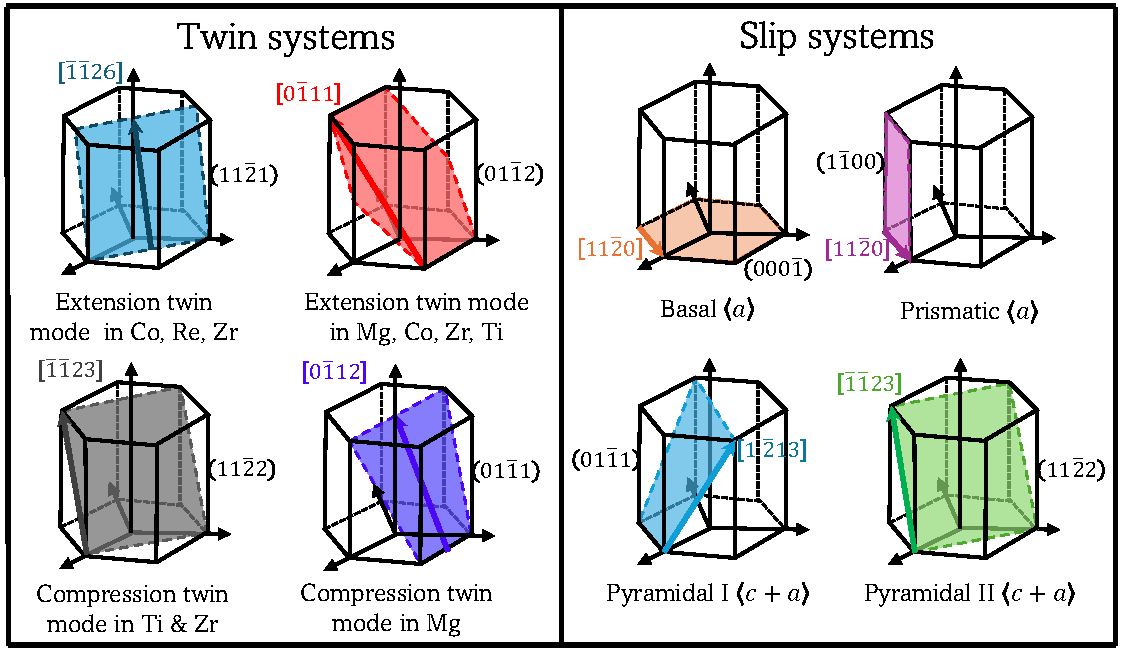
\includegraphics[width=\textwidth]{images/Slip_and_twin_systems.pdf}
    \caption{Commonly observed slip and twin Systems in HCP metals.}
    \label{HCP_Slip_Twin_Systems}
\end{figure}

The first 3 families operate in basal plane and provide only 4 independent slip systems and it is necessary to activate one of $\langle c+a \rangle$ slip systems or twin systems to meet the von Mises criterion \cite{taylor1938plastic} for arbitrary deformation. 

A twin mode or twin system can be described by four elements: undistorted plane $K_1$, the direction of shear $\eta_1$ and second undistorted plane $K_2$ and direction $\eta_2$. Since these 4 elements are interdependent, a twinning mode can be uniquely specified by either $K_1$ and $\eta_1$ or $K_2$ and $\eta_2$. Table \ref{Twin_systems} gives common twinning modes observed in various HCP metals. More details about twinning crystallography is presented in Chapter \ref{sec:twinning_crystallography}.

\begin{table}[H]
\centering
\caption{Commonly observed twinning modes in HCP metals.}
\renewcommand\arraystretch{1.2}
\renewcommand\baselinestretch{1.2}
\begin{tabular}{|c|c|c|c|}
\hline

$k_1$ plane & $\eta_1$ direction & Material \\
 \hline
 $\{10\Bar{1}2\}$ & $\langle 10\Bar{1}\Bar{1} \rangle$ & Cd, Zn, Co, Mg, Zr, Ti, Be  \\
 $\{10\Bar{1}1\}$ & $\langle 10\Bar{1}\Bar{2} \rangle$ & Mg, Ti  \\
 $\{11\Bar{2}2\}$ & $\frac{1}{3} \langle 11\Bar{2}\Bar{3} \rangle$ & Ti, Zr  \\
 $\{11\Bar{2}1\}$ & $\frac{1}{3}\langle \Bar{1}\Bar{1}2 6\rangle$ & Co, Re, Zr, Ti \\
 \hline
\end{tabular}

\label{Twin_systems}
\end{table}



\subsection{Computational Material Science}

The principle behind computational material science is that microstructural parameters determines the functional parameters. If we control the microstructure of the material we can improve the performance or properties of the materials. Figure \ref{Computational_materials} shows the schematic representation of the workflow in the computational material science.

\begin{figure}[H]
    \centering
    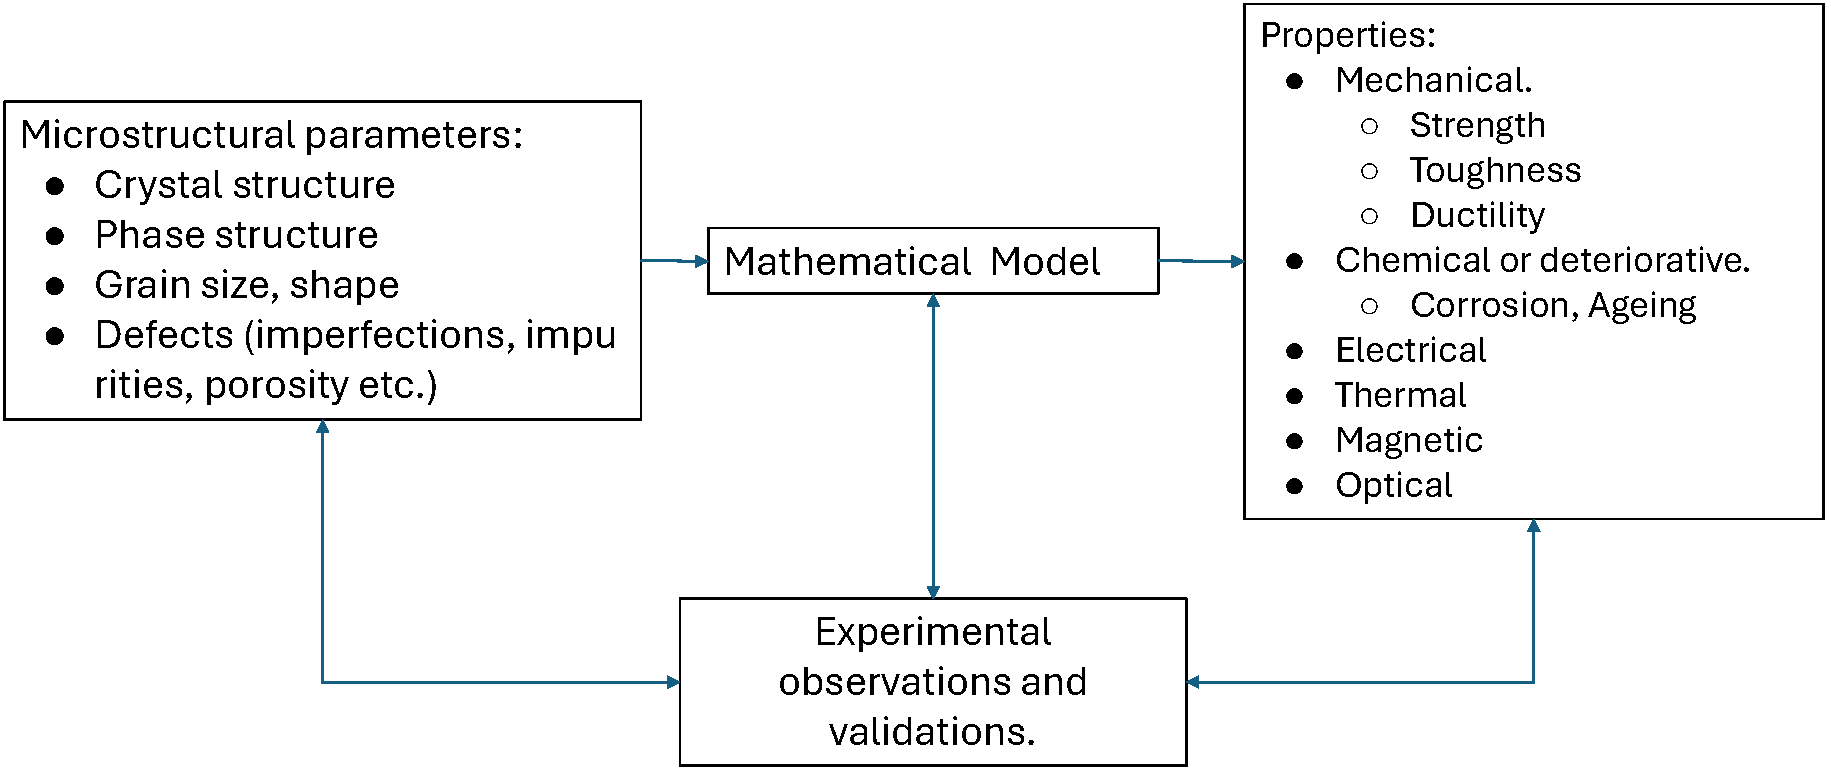
\includegraphics[width=\textwidth]{images/Computational_materials.pdf}
    \caption{Computational Material Science.}
    \label{Computational_materials}
\end{figure}

Computational material science uses the information from the experiments to observe and quantify the microstructural parameters and also to test the performance parameters of the materials. Table
\ref{Microstructural_parameter_exp_technique} adapted from Roters \cite{roters2011advanced} lists the experimental techniques that are used to measure microstructural parameters. 

At the heart of the computational material science is the mathematical model which is used to establish relationship between the microstructural parameters and defects to the performance parameters which are useful for engineering applications of the materials.

The \textbf{crystal plasticity} is the constitutive mathematical model which establishes relationship between the defects like dislocations and twinning with the mechanical properties like strength, ductility, toughness etc. 

\begin{table}[H]
\centering
\caption{Measurable quantities which can be predicted by CPFE models.}
\renewcommand\arraystretch{1.2}
\renewcommand\baselinestretch{1.2}
\begin{tabular}{|c|m{10cm}|}
\hline

  \textbf{Microstructural quantity} & \textbf{Experimental techniques/observations} \\
  \hline
  Dislocation dynamics & Flow stress measurement, transmission electron microscopy, lattice orientation measurements, electron channeling contrast imaging in the scanning electron microscope.  \\
  \hline
  Deformation twinning & Metallography, X-ray and synchrotron diffraction, electron backscatter diffraction, transmission electron microscopy, electron channeling contrast imaging in the scanning electron microscope. \\
  \hline
  Texture evolution & Texture measurements using electron diffraction in the transmission and scanning electron microscope(Kikuchi, SAD, CBED) or X-ray Bragg diffraction.  \\
  \hline
  Crystal Plasticity & Hardness testing, metallography, electrical resistivity, X-ray and synchrotron diffraction, electron backscatter diffraction, transmission electron microscopy, grain size determination, kernel average orientation determination, calorimetry.  \\

 \hline
\end{tabular}

\label{Microstructural_parameter_exp_technique}
\end{table}



\subsubsection{Crystal Plasticity}

\begin{wrapfigure}{rH}{0.45\textwidth}
    \centering 
    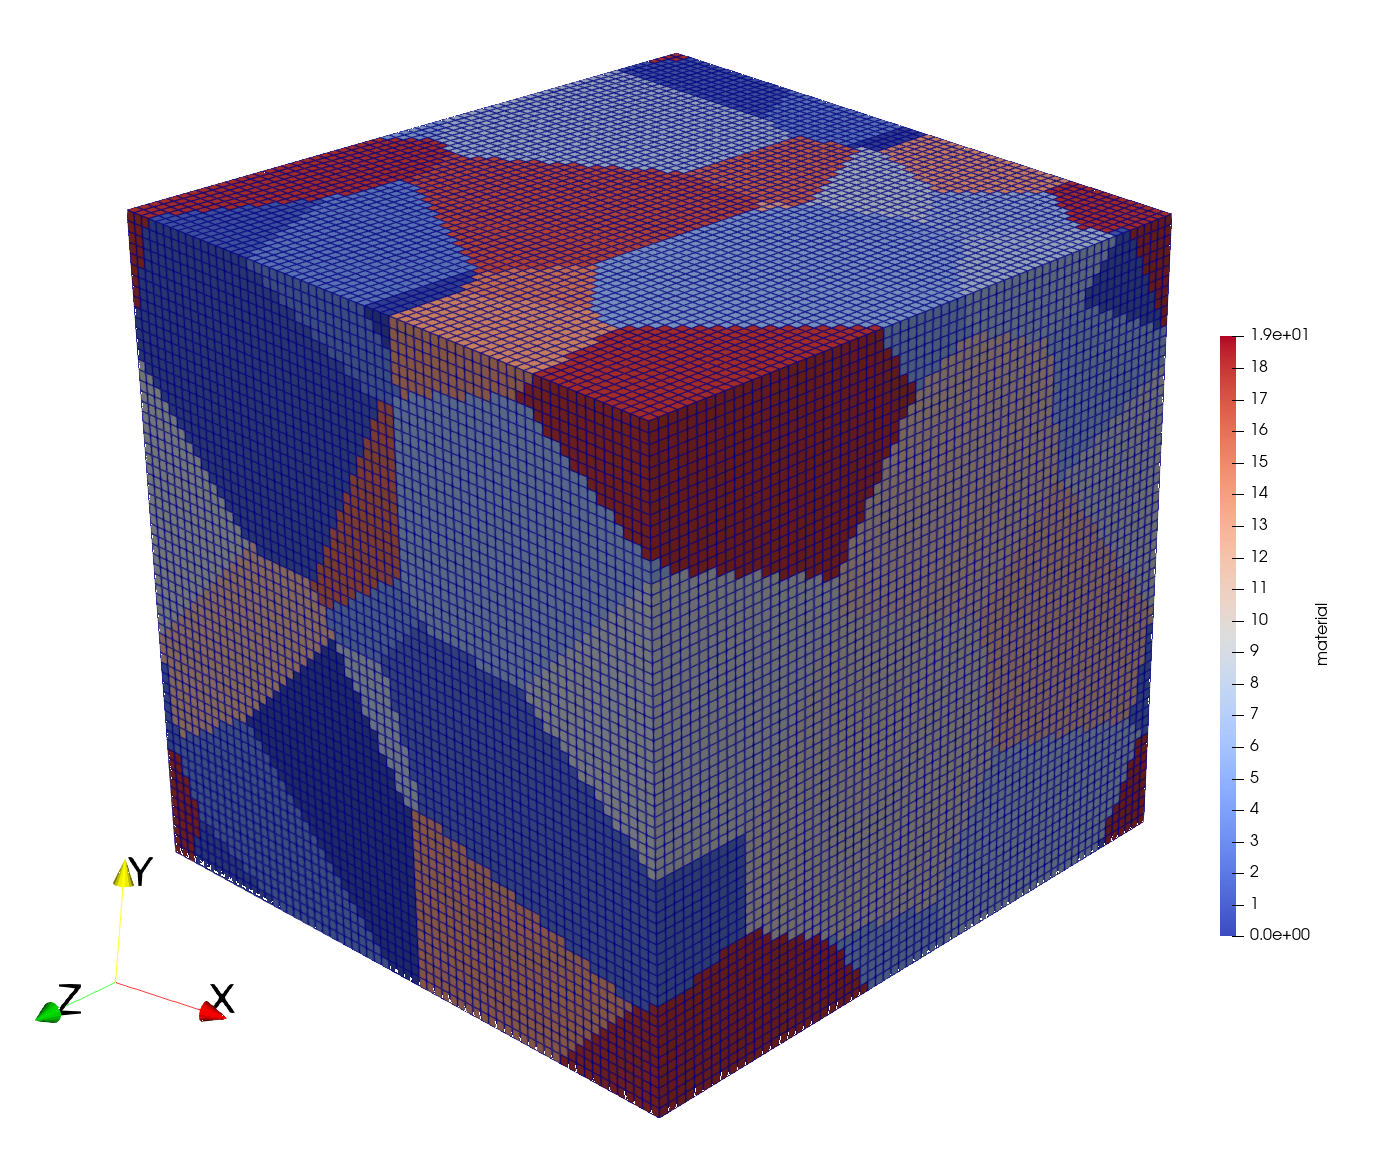
\includegraphics[width=0.4\textwidth]{images/RVE.png}
    \caption{A representative volume element with 20 grains.}
    \label{RVE}
\end{wrapfigure}

Crystal plasticity model is a constitutive mathematical model used to study deformation behavior of materials which are subjected to loads. It mainly contains 3 parts \cite{roters2011advanced}:

\begin{enumerate}
    \item Microstructure parameterization: We choose parameters in the microstructure which may affect the deformation behavior. Lattice parameters, isotropic/non-isotropic, Schmid factor, dislocation density etc.
    \item Laws for Microstructure Evolution Rates: Hardening laws, isotropic or kinematic, slip resistance, interaction matrix etc.
    \item Deformation kinetics: This is the part which connects the evolution of defects to the plastic deformation behavior by evaluating plastic deformation gradient.
\end{enumerate}

The crystal plasticity simulation is often done on a ``Representative Volume Element" which is a numerical representation of a polycrystal. An example RVE is shown in the figure \ref{RVE}



\vspace{2mm}
\textbf{Crystal Plasticity FEM/FFT:}

Most of the crystal plasticity models are formulated in the framework of continuum mechanics which is discussed in Appendix \ref{Appendix:Continuum_mechanics}. Figure below is the schematic of crystal plasticity in framework of continuum mechanics.

\begin{figure}[H]
    \centering
    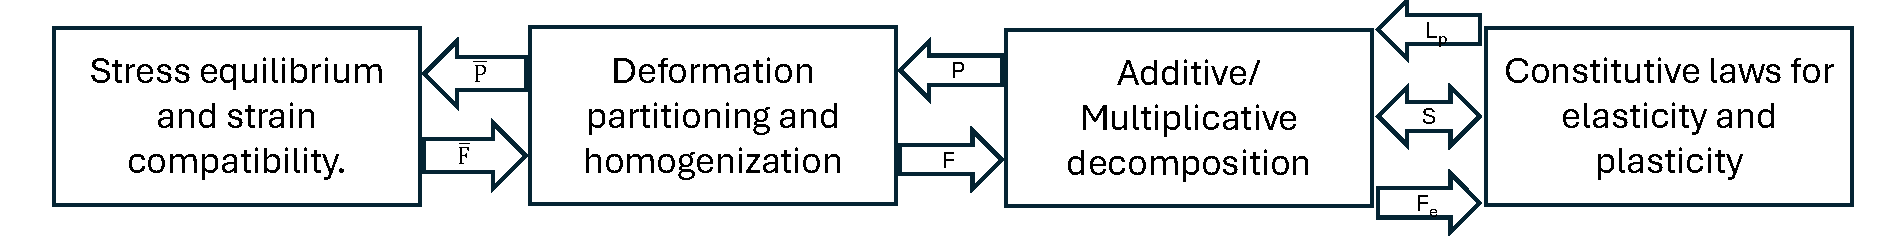
\includegraphics[width=\textwidth]{images/Typical_Crystal_Plasticity_model.pdf}
    \caption{A typical Crystal Plasticity scheme.}
    \label{Typical_CP_model}
\end{figure}

\textbf{Solution methodology:}

Solution methodology involves solving partial differential equations (PDEs) which describes the stress equilibrium. Most commonly used technique to solve the PDEs is ``Finite Element Method". If the boundary conditions are periodic and geometry is simple, solving the partial differential equations can be done using a faster alternative method ``Fast Fourier Transform(FFT)" or ``spectral solver". In our case, we use FFT solver to speed up the the process of model testing for which we consider simple test cases.

\subsubsection{Fast Fourier Transform Based ``Spectral Solver":}

The FFT method discretizes a microstructure on a regular grid in order to use Fast Fourier Transforms to solve the (partial) differential equations for stress Equilibrium.

\begin{table}[H]
\centering
\caption{Differences between FFT and FEM solvers.}
\renewcommand\arraystretch{1.2}
\renewcommand\baselinestretch{1.2}
\begin{tabular}{|m{4cm}|m{5.8cm}|m{4.5cm}|}
\hline
Criteria & Fast Fourier Transform solver & Finite Element solver \\
 \hline
Computational time & Order (Nlog2N) & Order (N2)  \\
 \hline
 Spatial arrangement of material points & Structured grid & Depends on mesh (affects convergence)  \\
  \hline
 Boundary conditions & Homogeneous stress or strain rate (force and displacement now possible via non-periodic FFTs) & Forces and displacements \\
  \hline
 Domain & Periodic Representative Volume Element (although efficient non-periodic FFTs exist) & Any shape and size \\
  \hline
 Interfaces & Not well defined (has its advantages/disadvantages) & Well-defined (has its advantages/disadvantages) \\
  \hline
 Dimensions & 2D/3D full field & 2D/3D full field \\
  \hline
 Large deformations & Computations done in reference configuration & Computations in reference and current configurations \\
 \hline
\end{tabular}

\label{Differences between FFT and FEM solvers}
\end{table}

The method utilizes the fact that the local response of a heterogeneous medium can be calculated using convolution integrals. These integrals involve Green's functions, which represent the micromechanical fields of an equivalent linear homogeneous medium with eigenstrains, and a polarization field. The polarization field captures the actual heterogeneity of the medium, including any potential non-linear behavior of the local mechanical properties. In simpler terms, the approach decomposes the heterogeneous medium into two components: an equivalent homogeneous medium with eigenstrains (captured by Green's functions) and a polarization field that accounts for the deviations from homogeneity, such as local variations in material properties or non-linear behavior. By convolving these two components, the local response of the heterogeneous medium can be computed accurately.

The below figure \ref{FFT Solution procedure} shows the steps involved in FFT solver:
\begin{figure}[H]
    \centering
    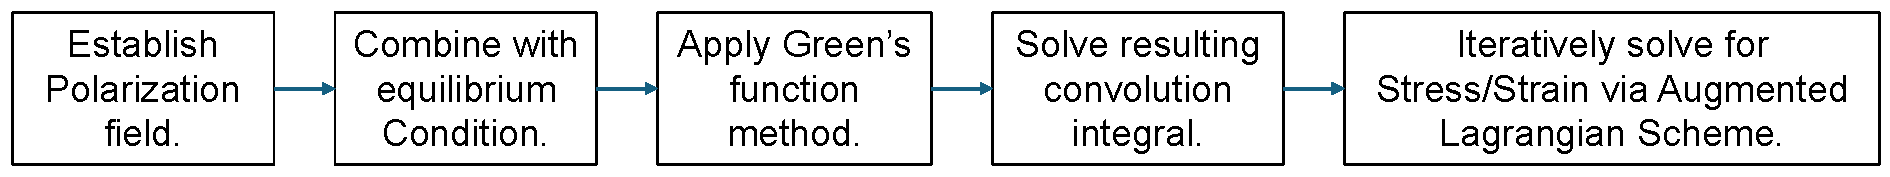
\includegraphics[width=\textwidth]{images/FFT solution procedure.pdf}
    \caption{FFT solution procedure.}
    \label{FFT Solution procedure}
\end{figure}

Fast fourier transform, when compared with FEM, saves on computational effort and time, hence it is used to solve equilibrium equations derived from the crystal plasticity model. The table \ref{Differences between FFT and FEM solvers} shows the differences between FFT and FEM.




